\documentclass{beamer}
\usepackage[utf8]{inputenc}

\usetheme{Madrid}
\usecolortheme{default}
\usepackage{amsmath,amssymb,amsfonts,amsthm}
\usepackage{txfonts}
\usepackage{tkz-euclide}
\usepackage{listings}
\usepackage{adjustbox}
\usepackage{array}
\usepackage{tabularx}
\usepackage{gvv}
\usepackage{lmodern}
\usepackage{circuitikz}
\usepackage{tikz}
\usepackage{graphicx}
\usepackage{gensymb}

\setbeamertemplate{page number in head/foot}[totalframenumber]

\usepackage{tcolorbox}
\tcbuselibrary{minted,breakable,xparse,skins}



\definecolor{bg}{gray}{0.95}
\DeclareTCBListing{mintedbox}{O{}m!O{}}{%
  breakable=true,
  listing engine=minted,
  listing only,
  minted language=#2,
  minted style=default,
  minted options={%
    linenos,
    gobble=0,
    breaklines=true,
    breakafter=,,
    fontsize=\small,
    numbersep=8pt,
    #1},
  boxsep=0pt,
  left skip=0pt,
  right skip=0pt,
  left=25pt,
  right=0pt,
  top=3pt,
  bottom=3pt,
  arc=5pt,
  leftrule=0pt,
  rightrule=0pt,
  bottomrule=2pt,
  toprule=2pt,
  colback=bg,
  colframe=orange!70,
  enhanced,
  overlay={%
    \begin{tcbclipinterior}
    \fill[orange!20!white] (frame.south west) rectangle ([xshift=20pt]frame.north west);
    \end{tcbclipinterior}},
  #3,
}
\lstset{
    language=C,
    basicstyle=\ttfamily\small,
    keywordstyle=\color{blue},
    stringstyle=\color{orange},
    commentstyle=\color{green!60!black},
    numbers=left,
    numberstyle=\tiny\color{gray},
    breaklines=true,
    showstringspaces=false,
}
\begin{document}

\title 
{4.7.26}
\date{September 19,2025}


\author 
{Kishora Karthik-EE25BTECH11034}
\frame{\titlepage}
\begin{frame}{Question}
Find the equation of a straight line on which length of perpendicular from the origin is four units and the line makes an angle of $120\degree$ with the positive direction of X-axis.
\end{frame}

\begin{frame}{ Solution}
Let $p$ be the length of perpendicular from the origin and $\theta$ be the angle made by the line with the positive X-axis.\\
Given, $p=4$ and $\theta=120\degree$.
Let the angle made by the perpendicular with the positive X-axis be $\alpha$.
\begin{align}
    \alpha=90\degree-(180\degree-\theta)
\end{align}
\begin{align}
    \alpha=90\degree-(180\degree-120\degree)
\end{align}
\begin{align}
    \alpha=30\degree
\end{align}
$p\myvec{ \cos\alpha \\ \sin\alpha }$
is a point on the line as well as the normal vector. Hence the equation of the line is,
\begin{align}
p\myvec{ \cos\alpha \\ \sin\alpha}^\top\brak{\vec{x} - p  \myvec{ \cos\alpha \\ \sin\alpha}}   = 0
\end{align}
\end{frame}

\begin{frame}{Solution}
\begin{align}
\implies p\myvec{ \cos\alpha & \sin\alpha}\brak{\vec{x} - p  \myvec{ \cos\alpha \\ \sin\alpha}}   = 0
\end{align}
\begin{align}
\implies  p\myvec{ \cos\alpha & \sin\alpha}\vec{x} = p^2(\cos^2\alpha+\sin^2\alpha) 
\end{align}
\begin{align}
\implies  \myvec{ \cos\alpha & \sin\alpha}\vec{x} = p 
\end{align}
So the equation of the straight line is,
\begin{align}
\myvec{ \cos30\degree & \sin30\degree}\vec{x} = 4 
\end{align}
\end{frame}
\begin{frame}{Solution}
\begin{align}
\myvec{ \frac{\sqrt{3}}{2} & \frac{1}{2}}\vec{x} = 4 
\end{align}
$\therefore$ The equation of the required line is $\myvec{ \frac{\sqrt{3}}{2} & \frac{1}{2}}\vec{x} = 4$ or ${\sqrt{3}}x + y=8$.
\end{frame}
\begin{frame}{Plot}
    \centering
    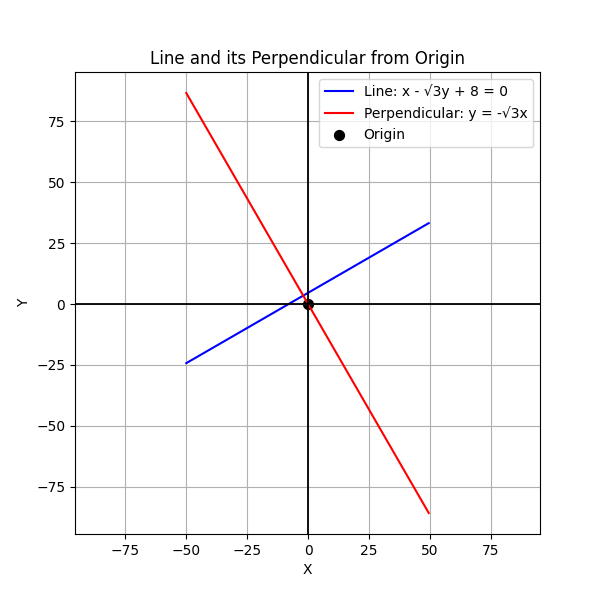
\includegraphics[width=\columnwidth, height=1\textheight, keepaspectratio]{figs/fig1.png} 
\end{frame}

\end{document}



